\documentclass{article}
\usepackage[english]{babel}
\usepackage{amsthm, amssymb}
\usepackage{graphicx}
\usepackage{hyperref}
\graphicspath{ {./images/} }

\theoremstyle{theorem}
\newtheorem{theorem}{Theorem}[section]
\theoremstyle{definition}
\newtheorem{definition}{Definition}[section]
\theoremstyle{example}
\newtheorem{example}{Example}[section]
\theoremstyle{proposition}
\newtheorem{proposition}{Proposition}[section]

\begin{document}
    \begin{center}
        \Large
        \textbf{Expander Graphs}

        \vspace{0.4cm}
        \large
        Introduction for Mathematics Minors
        
        \vspace{0.4cm}
        \textbf{Karen Arzumanyan}

        \vspace{0.2cm}
        November 28, 2021

    \end{center}

    \begin{abstract}
        The following paper deals with the important concept of expander graphs and its main characteristics. Starting from the very basic definition of a graph, and building up until the celebrated Cheeger Inequality, we created a quite self contained introductory work to the field of expander graphs. Most of the results are provided with rigorous proofs, and are illustrated by various examples. While preparing the current manuscript, we mainly aimed to help the reader with no prior knowledge in graph theory to enter the scientific area of expander graphs.
    \end{abstract}

    \section{Introduction}
        For people who are not as deep into mathematics as someone who studies it professionally, many unknown concepts may seem very difficult and tedious to understand. One such concept is \textit{graphs}, more specifically, \textit{expander graphs}. To some, this topic may seem like a horizon never explored, and some may even believe that it is best to leave it that way. However, in reality, the concept of an expander graph is very interesting and is definitely worth exploring, especially if one is involved in \textit{Computer Science }and \textit{Information Theory}.

    By an expander graph we understand a graph that is connected. This does seem very vague indeed, but it is difficult to summarize the concept of an Expander Graph in a few sentences, such that it is understandable while remaining true to the concept.

    Imagine a bunch of cities that are connected to each other, and each city has a highway connecting it to a fixed number of other cities. We know that each city is connected on the grid, and there is always a path between two random cities.

    Let us consider an example of a resident of one of the cities who is planning to have a roadtrip, but does not care to which city they travel. For the sake of the argument, suppose that each city is connected to 6 other cities. To determine the next city to visit, the person throws a fair die and goes to the connected city decided by the die. Using mathematical language, we can say that in this case each random decision is \underline{\emph{uniform and independent of the previous ones}}. This is an example of a random walk on an expander graph. The described property of uniformity and independence are two crucial features of random walks on expanders.
    It is not hard to find the probability of the person arriving to a certain desired city. Additionally, suppose that the person decides to have a large number of roadtrips. Everytime they arrive at another city, they throw the die again, and go to the neighbor decided by the die. If the number of roadtrips exceeds the number of cities by a large amount, then the person would pass some if not all of the cities multiple times.
    In this example, the cities can be considered as the vertices of a graph with the highways being the edges.

    This paper introduces the important notions of basic graph theory and its interaction with linear algebra. Our main interest will be a clear of the concept of an expander graph. Those graphs are of great imporance in both theoretical and practical senses. Although, our paper is mostly of theoretical nature, the examples below show the practical imporance of expander graphs.
    
        \begin{description}
            \item[Reduction of the need for Randomness:] Expanders can be used to reduce the number of random bits needed to make a probabilistic algorithm work with some desired probability.
            \item[Finding good error-correcting codes:] Expanders can be used to construct error correcting codes for protecting information against noise. Expanders can be used to find error correcting codes which are efficiently encodable and decodable. Finding codes with such properties was one of the milestone in information theory.
        \end{description}

        There are many more applications of expanders in fields such as \textit{Mathematics} and \textit{Information Theory}, with many more to be discovered. Thus, giving one who is confident when working with \textit{Expander Graphs} an upper hand in the engineering industry.

        In the following sections, we introduce and discuss the concepts of graphs, expansion parameters, expander graphs, adjacent matrices and their eigenvalues, and the Cheeger inequality.
        Our sources include the works of \cite{N} and \cite{G} with \cite{N} being the main work that we are referring to.

    \section{Graphs}
        A graph in mathematics is a collection of vertices which are connected through edges. Using the example with the cities, each city is a vertex, and the roads connecting the cities together are edges.
        \begin{definition}[Graphs]
            A graph $G$ is determined by a set $V$ of vertices, and a set $E$ of edges which connect the elements of $V$ to each other.  An edge $e \in E$ which connects $v_1,v_2 \in V$ is denoted by $(v_1, v_2)$.
        \end{definition}

        \newpage
        \begin{example}
            The figure represents a graph with vertices $V = \{A,B,C,D,E,F\}$ and edges $E = \{(A,B), (A,C), (A,C), (B,D), (C,F), (E,F)\}$
            \begin{figure}[h]
                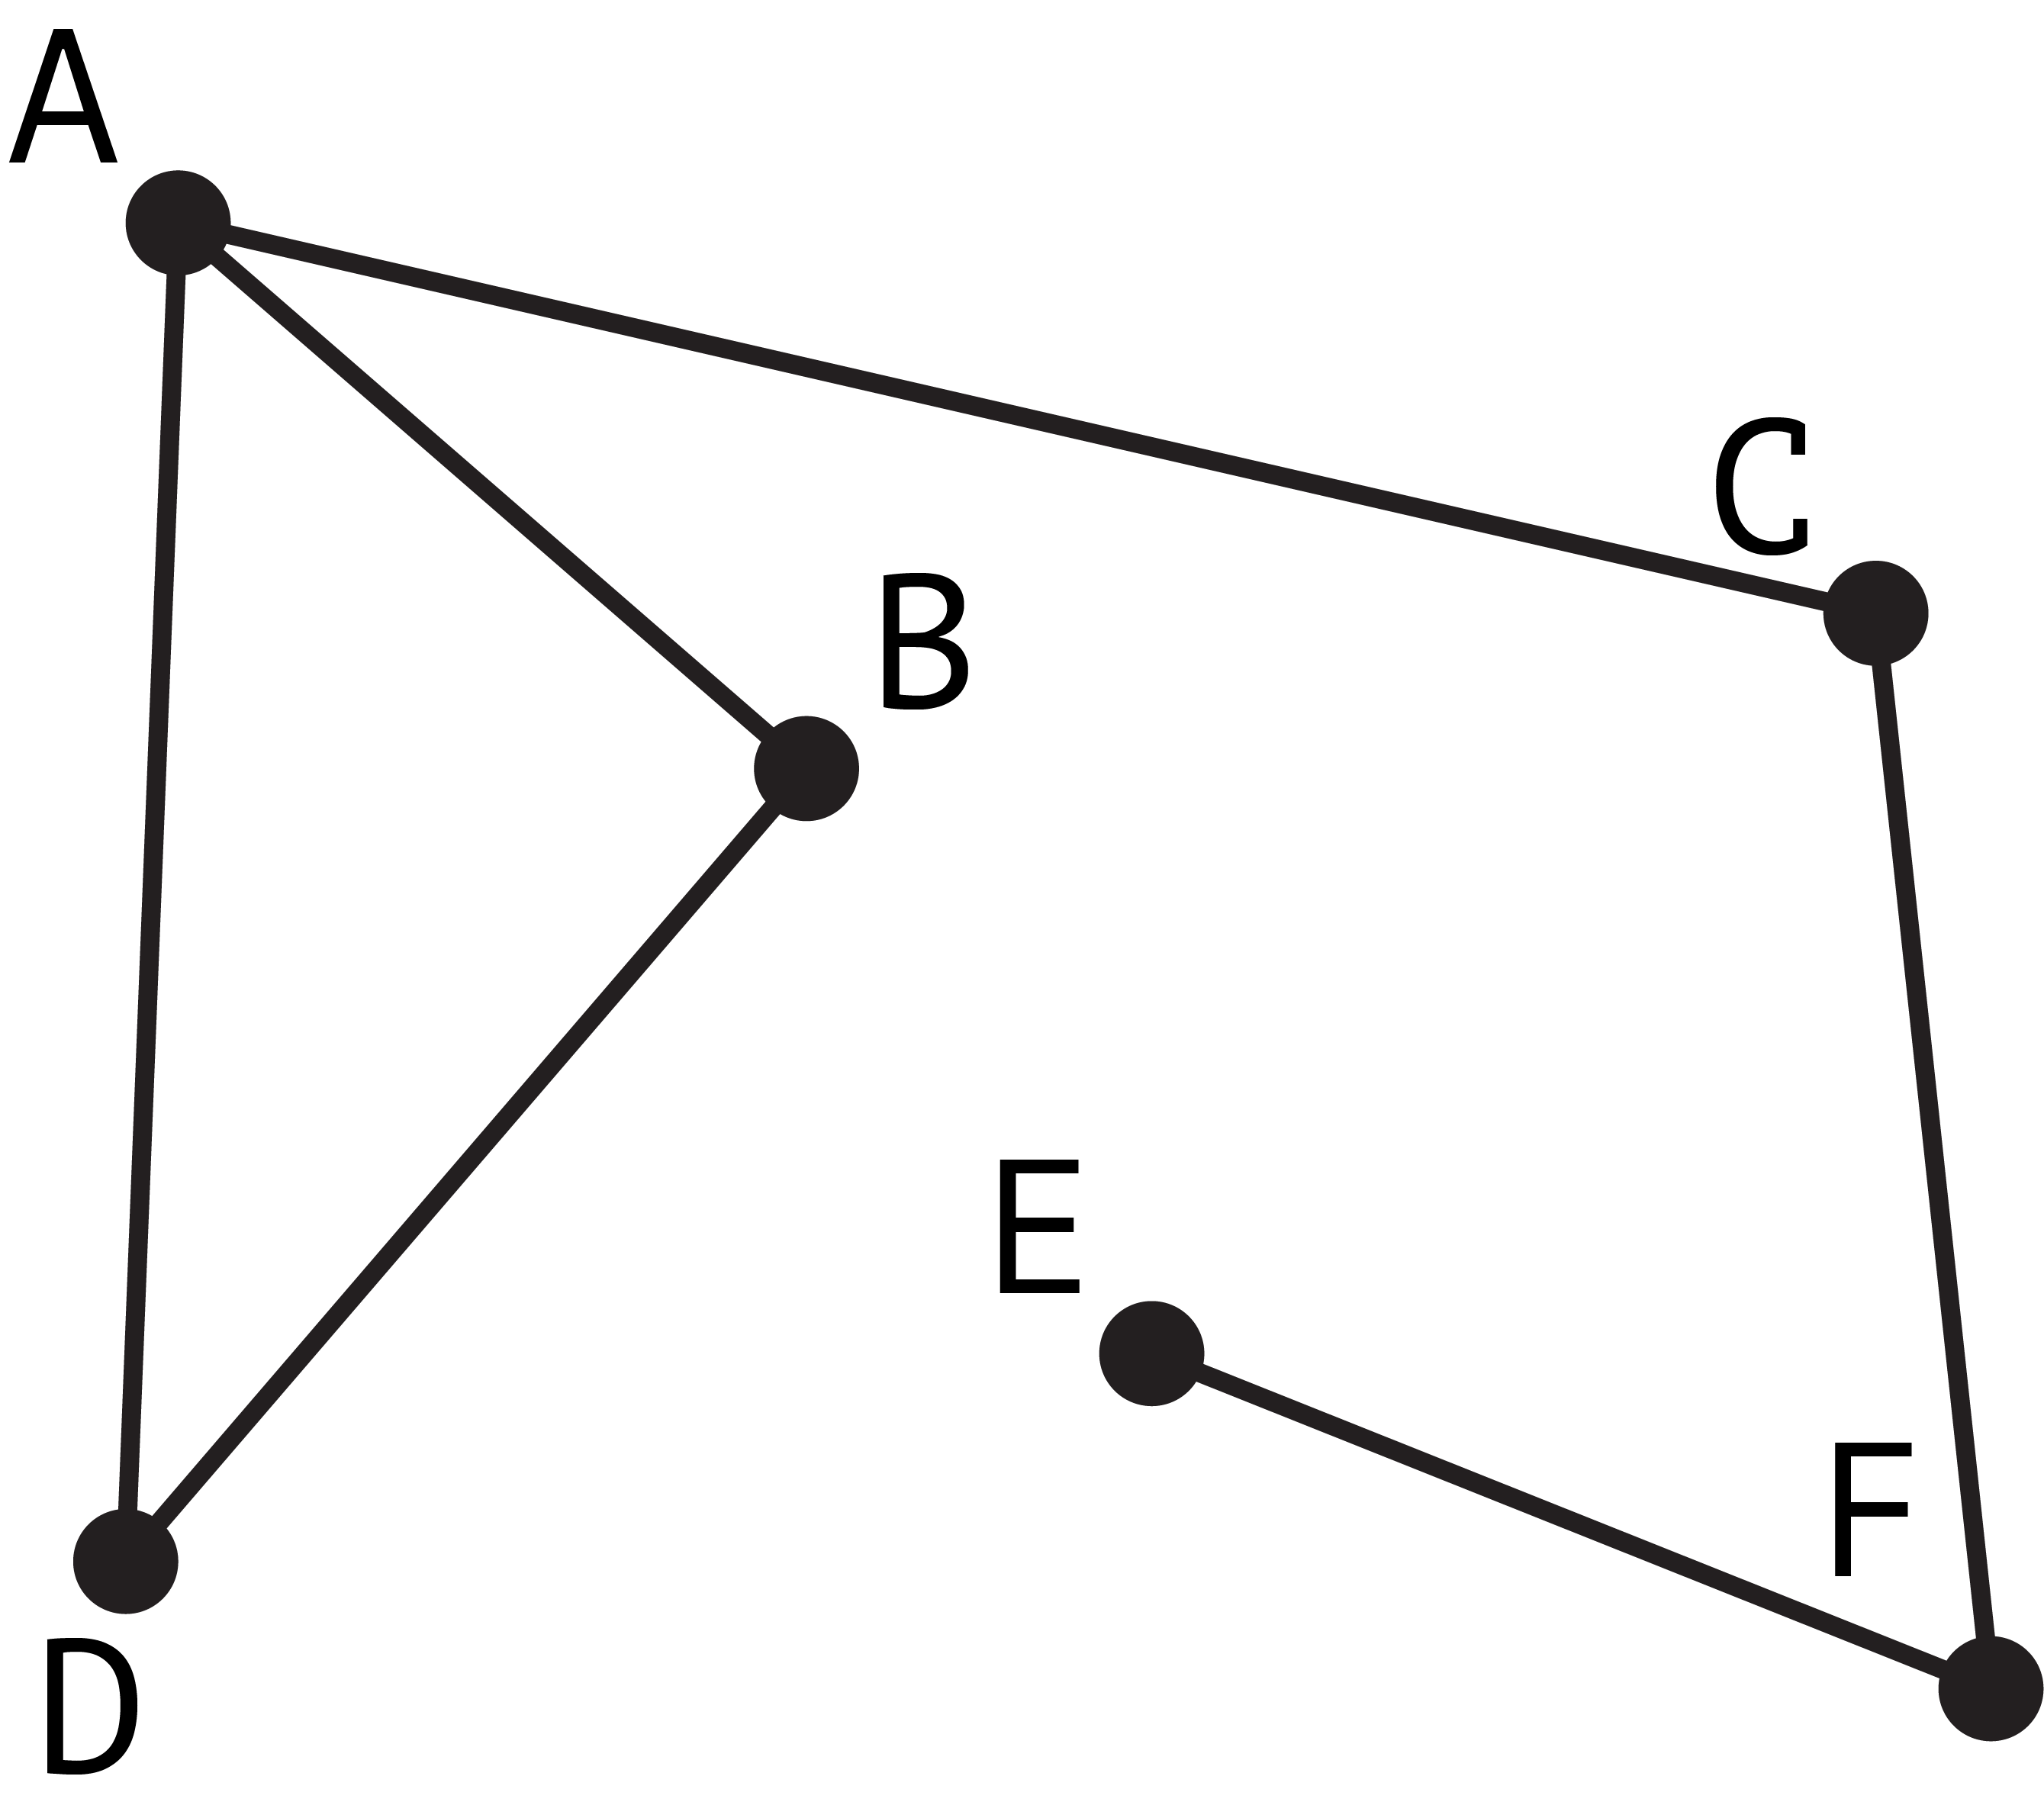
\includegraphics[width=5cm]{Graph.png}
                \centering
            \end{figure}
        \end{example}

        Unlike the example with the cities, where we stated that each city (vertex) connects to a constant number of other vertices, in this graph, vertices connect to different number of vertices. For example, $A$ connects to $3$, while $E$ only connects to one.
        A graph does not have to have its vertices connect to a constant number of other vertices, however, when a graph does poses that property, it is called a \textit{d-regular} graph.
        \begin{definition}[\textbf{\textit{d-regularity}}]
            A graph $G$ is called \textit{d-regular} if and only if every $v \in V$ is connected to $d$ other vertices in $V$.
        \end{definition}

        It is possible to turn the graph drawn above into a \textit{d-regular} graph.
            \begin{figure}[h]
                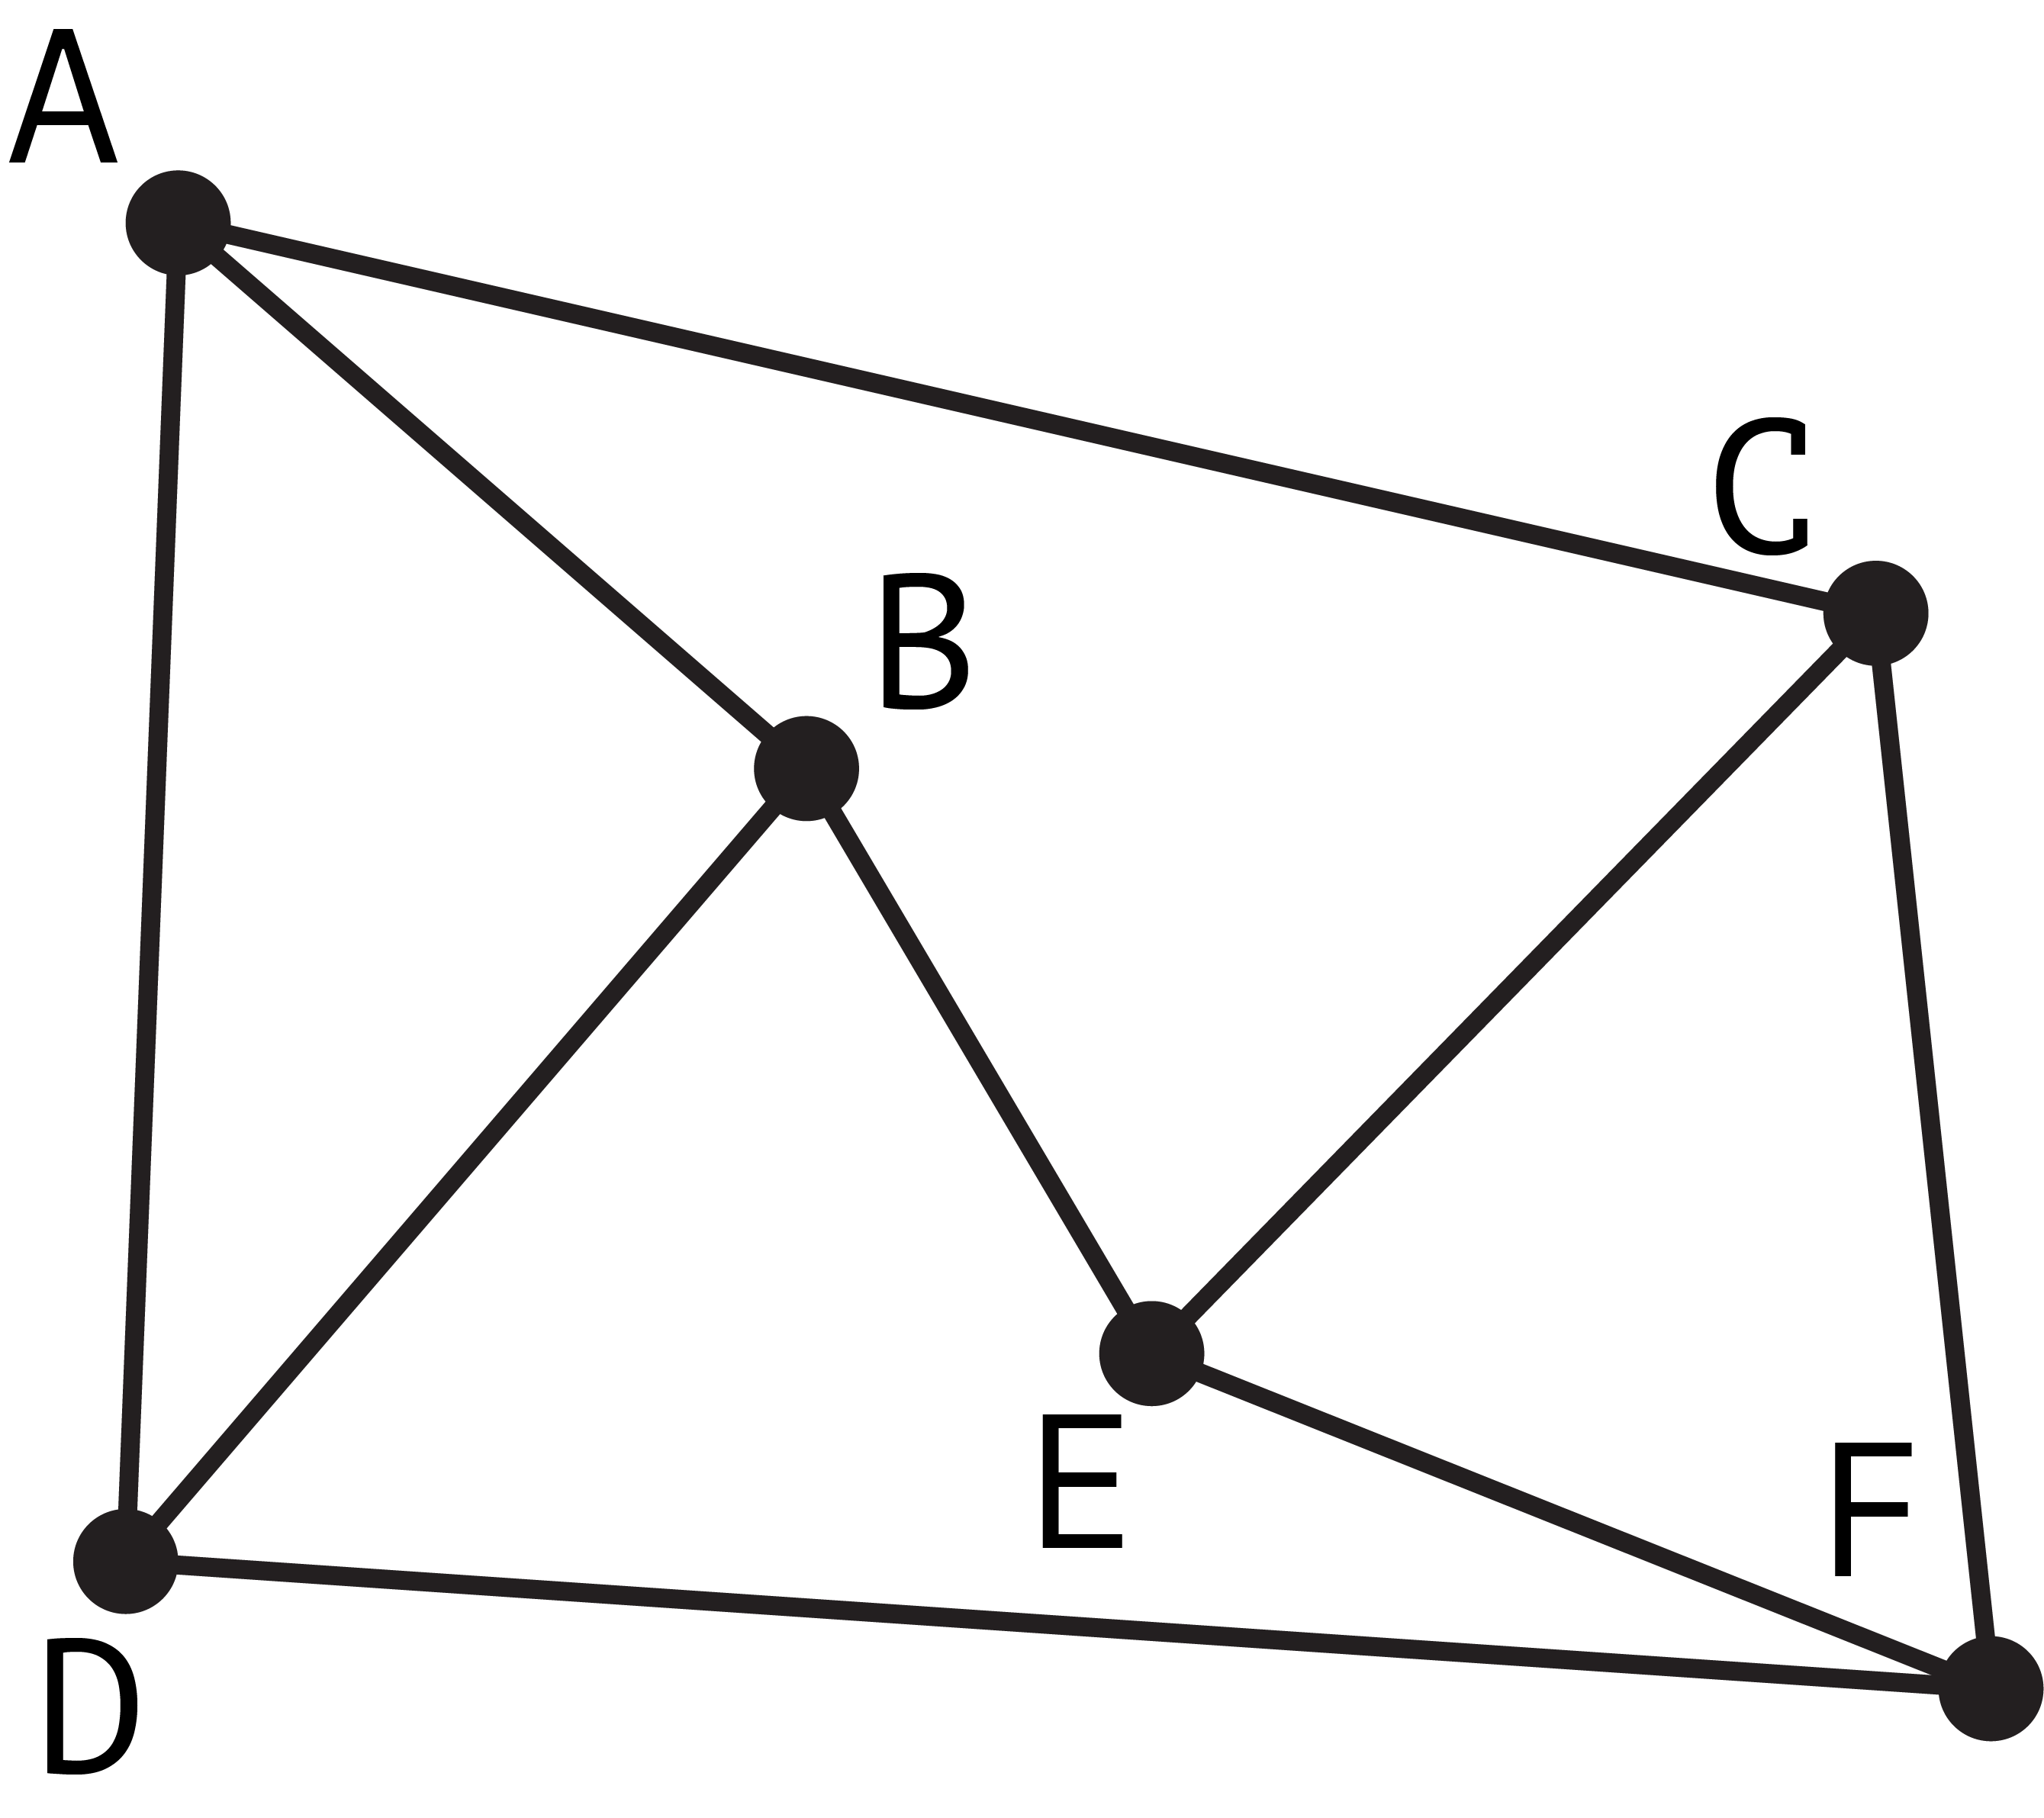
\includegraphics[width=5cm]{dGraph.png}
                \centering
            \end{figure}
        Now, each vertex in the graph connects to $3$ other vertices. This makes the graph \textit{$3$-regular}.
        Knowing the definition of a Graph, \textit{d-regularity}, it is only left to understand connectivity until we are able to define an Expander Graph. Put in simple words, a graph $G$ is a connected graph, if there exists a path between two random vertices, i.e, each vertex in the graph is connected to every other vertex either directly or through other vertices.
        Now, it is time to give a definition for an expander graph, albeit an informal one.
        \begin{definition}[\textbf{Informal Expander Graphs}]
            A \textit{d-regular} Graph $G = (V,E)$ is called an \textit{expander graph} if and only if every $S \subset V$ has its vertices connected to many vertices in $\bar{S} \subset V$. Where $\bar{S} = V - S$.
        \end{definition}
        Again, sounds vague, doesn't it? What exactly does it mean to connect to ``many'' vertices, one might ask. We will explore the meaning of the phrase "many vertices," but first, we should explore the concept of expansion.

    \section{Expansion}
        Expansion of a graph is measured using the \textit{Expansion Parameter} also known as the \textit{Cheeger Constant}. In a way, it measures the minimum ratio between $S \subset V$ and its \textit{Edge Boundary}.
    \begin{definition}[\textbf{Edge Boundary}]
        For a subset $S$ of $V$, we define the \textit{edge boundary} of $S \subset V$ to be the set of edges connecting $S$ to its complement $\bar{S}$. We write the \textit{edge boundary} of $S$ as $\partial{S}$
        $$\partial{S} = \{(v,w) | v \in S \textit{ and }  w \not\in S\} \subset E$$
    \end{definition}
        A way to understand \textit{edge boundary} using the city analogy, is to imagine a \textit{d-regular} connection of cities; however, let's pick a few cities and consider them a part of a state. That will be our subset $S$, we know that there are highways connecting those cities to each other in the state; however, there are also highways connecting the cities from the state to the cities outside of the state. The set of those highways, is exactly our edge boundary. In other words, if a road connects a city in the state to one outside of the state, is part of the \textit{edge boundary}.
        Using the defintion of the edge boundary, we can now define the Expansion Parameter of a graph.
        \begin{definition}[\textbf{Expansion Paramter}]
            We define the \textit{expansion parameter} as a  function
            \[h(G) \equiv \min\limits_{S:|S| \leq \frac{n}{2}} \frac{|\partial{S}|}{|S|}\textrm{.}\]
            $h(G)$ is the smallest possible ratio between the size of the \textit{edge boundary} of $S \subset V$ and the size of $S$, where we constrain $|S| < \frac{n}{2}$.
        \end{definition}
        It is helpful if we consider a few examples of graphs and try to calculate their \textit{expansion parameter} However, we will from this point on leave the analogy of the cities, and provide the examples in a mathematical form.
        \newpage
        \begin{example}
            Suppose $G$ is a graph consisting of $n$ vertices, such that each vertex is connected to every other vertex (also known as a complete graph). Then for any two vertices $v \in S$ and $w \in \bar{S}$ there exists an edge $e \in E$ such that $e = (v,w)$.
            
            Since the graph consists of $n$ vertices, then the the set complement of $S$ consists of exactly $n-|S|$ vertices.
            We also know that each vertex in $S$ connects to all the vertices in $\bar{S}$, so there are exactly $|S| \times |\bar{S}|$ edges in $\partial{S}$.

            Thus, we can compute that $|\partial{S}| = |S| \times |\bar{S}| = |S|(n-|S|)$.

            Now, if we substitute our findings into $h(G)$ we get,
            \[h(G) = \min\limits_{S:|S| \leq \frac{n}{2}} n - |S|\]
            The expression $n - |S|$ is at its minimum when $|S|$ is at its maximum, so we substitute $\Big\lceil{\frac{n}{2}}\Big\rceil$ instead of $|S|$ and get
            \[h(G) = \Big\lceil{\frac{n}{2}}\Big\rceil\]
        \end{example}

        %Possible example picture?
        
        Before proceding to the next example, we need to understand a property of a lattice (which is only relevant to the next particular example and not to expander graphs in general).

        \textit{Periodic boundary condition} of a finite lattice graph is a way to ``eliminate'' its finiteness. Without going into detail, suppose we have a $3 \times 3$ square lattice where every point connects to the one above, below, to the left, and to the right, imposing a \textit{periodic boundary condition} on it will result in the edge points being layered ontop of the edge points on the opposite sides by wrapping. Basically, suppose we wish to go left from one of the edge points on the left, we cant, because there is no point to the left anymore. However, with the periodic boundary, we can in fact go left, and we will arrive on the point left to the rightmost point on that row. A good way to visualize, is to imagine the lattice wrapped around a cylinder such that the edge points overlap. But that is only in the horizontal axis, if we add the condition on the vertical axis as well, then the whole lattice will be wrapped around a torus.
            \begin{figure}[h]
                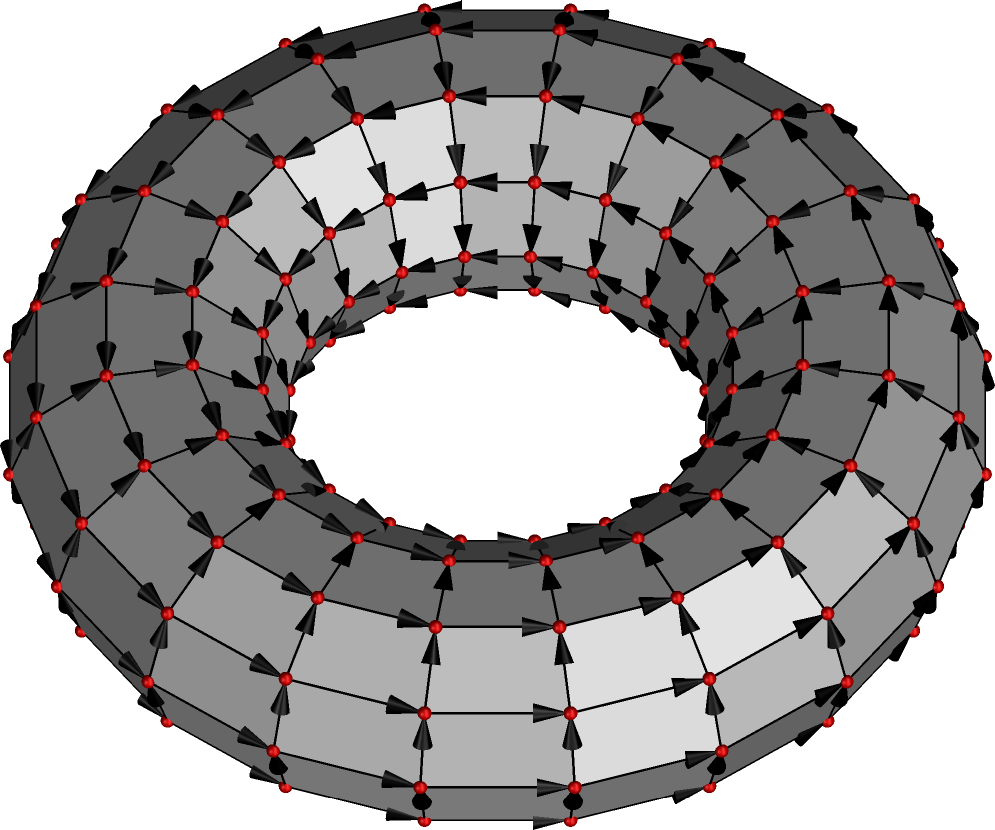
\includegraphics[width=5cm]{iu.png}
                \centering
            \end{figure}

            \newpage
            So we may pick a random point and be able to go to the left forever, and passing the initial point while doing so. And the same works when going the other directions.


            Knowing the above condition of a lattice, we will now give an example of a graph using a square lattice.
        \begin{example}
            Suppose that $G$ is an $n \times n$ lattice in 2 dimensions, with periodic boundary conditions (such that the graph becomes \textit{4-regular}. Then if we consider a large connected subset $S \subset V$, it ought to be plausible that the \textit{edge boundary} set $\partial{S}$ will contain roughly one edge for each vertex on the perimeter of the region S. We expect there to be roughly $\sqrt{|S|}$ such vertices.

            Thus
            \[\frac{|\partial{S}|}{|S|} \approx \frac{\sqrt{|S|}}{|S|} = \frac{1}{\sqrt{|S|}}\]
            Since the lattice is a square, we know that the subset $|S|$ may contain up to $O(n^{2})$ elements.

            Therefore,
            \[h(G) = O(\frac{1}{n})\]
            \textbf{Remark:} In this example, $\lim\limits_{n \rightarrow \infty} h(G) = 0$, which makes this graph a non-expander graph, for reasons we will see later.
        \end{example}
        
        \begin{example}
            Consider a \textit{d-regular} graph $G$. Let all vertices in $V$ be connected to d other \textit{random} vertices. Let $S \subset V$ consist of at most $\frac{n}{2}$ vertices. Since a vertex $v \in S$ connects to $d$ other vertices, and the probability of it connecting to a vertex in $\bar{S}$ is $\frac{|\bar{S}|}{n}$, then $v$ connects to $d \times \frac{|\bar{S}|}{n}$ vertices in $\bar{S}$.

            We expect $\frac{|\partial{S}|}{|S|} \approx \frac{1}{|S|} \times d\frac{|S| \times |\bar{S}}{n} = d\frac{|\bar{S}}{n}$

            Since $|\bar{S}|$ has its minimum at approximately $\frac{n}{2}$, we plug that value into $h(G)$ and get
            \[h(G) \approx d\frac{|\bar{S}|}{n} = d\frac{n}{2} \times \frac{1}{n} = \frac{d}{2}\]
            \[h(G) \approx \frac{d}{2}\]
        \end{example}

        It is important to note, that in each of our examples, we haven't constructed just a single graph, but rather a family of graphs, which were indexed by some parameter $n$, with a property that as $n$ get larger, so does the number of vertices in the graph.

        Now that we understand the expansion parameter, we are finally able to define what exactly is an \textit{expander graph}.

        \section{Expander Graphs}
        \begin{definition}[\textbf{Expander graphs}]
            If we have a family $G_j = (V_j, E_j)$ of \textit{d-regular} graphs, indexed by $j$, and such that $|V_j| = n_j$ for some increasing sequence $n_j$. Then we say that the family $\{G_j\}$ is a family of expander graphs if the edge expansion parameter is bounded strictly away from 0, i.e., there is some (small) constant $c$ such that $h(G_j) \geq c > 0$ for all $G_j$ in the family.
        \end{definition}
        
        Given the definition, we will now consider an example of an expander graph which will require some basic knowledge of Number Theory.
        \begin{example}
            Consider a family of graphs indexed by a prime number $p$. The set of vertices for the graph $G_p$ is just the set of congruence classes in $\mathbb{Z}_p$ (the field of integers modulo $p$). We can construct a \textit{3-regular} graph by connecting each vertex $x \not= 0$ to $x-1$, $x+1$, and $x^{-1}$ (it's multiplicative inverse in $\mathbb{Z}_p$.
            We will explicitly connect the vertex $x = 0$ to $p - 1$, $0$, and $1$
            We will explicitly connect the vertex $x = 0$ to $p - 1$, $0$, and $1$.
            This is proven to be a family of expander graphs by \textit{Lubotsky, Philips, and Sarnak} in 1988.
        \end{example}

        But how can \textit{we} prove that a family of graphs is an \textit{expander}?
        A way to show this is to calculate the ratio of $\frac{|\partial{S}|}{|S|}$ for every subset $|S|$ of vertices containing no more than half the vertices in the graph. But this is too time consuming, and since there are $n$ vertices in the graph, then there will be exponentially many such subsets $S$.
        Fortunately, graph theory and linear algebra are not full disjoint.

        \section{Adjacency Matrix of a Graph}
        An \textit{adjacency matrix} of a graph G, is a way for us to look at the connections of a graph. However, the marvel of it all, is that the \textit{eigenvalue spectrum} of the \textit{Adjacency Matrix} of a graph can be used to understand the properties of the graph $G$.

        But first, what exactly is an \textit{Adjacency Matrix}?
        \begin{definition}
            The rows and columns of the Adjacency Matrix are labelled by the vertices of V.

            More precisely, A(G) is the adjacency matrix of the graph $G = (V,E)$.
            Then for vertices $v,w \in V$, the entry $A(G)_{vw} = 1$ if $(v,w)$ is an edge, i.e. $(v,w) \in E$; likewise, $A(G)_{vw} = 0$ if $(v,w)$ is not an edge, i.e. $(v,w) \not \in E$.
        \end{definition}

        Given the above defintion, let's assume that we have a finite graph $G$ with $n$ vertices, then $A(G)$ is an $n \times n$ symmetric matrix. This implies that $A(G)$ has $n$ real \textit{eigenvalues}, counting multiplicities.
        \[\lambda_1 \geq \lambda_2 \geq \ldots \geq \lambda_n\]

        Furthermore, if $G$ is \textit{d-regular}, then the largest eigenvalue of $A(G)$ is $d$.

        The proof of the above statement is quite simple.
        \newpage
        \begin{proof}
            Suppose we have a finite \textit{d-regular} graph G of size $n$. Then the \textit{adjacency matrix} is a symmetric $n \times n$ matrix.
            Since the graph is \textit{d-regular}, then each row of the \textit{adjacency matrix} will have exactly $d$ 1s.
            If we take the vector $\vec{1}$ (a vector of dimension $n$ with all entries $1$), and multiply it with the matrix, we will get $d \vec{1}$, which is an $n$ dimensional vector with all entries $d$.
        \end{proof}

        Now that we have an idea of how we connect the \textit{adjacency matrix} to a graph, let's define a simple concept.
        \begin{definition}[Spectrum of a Graph]
            The spectrum of a graph $G$ is the set of all \textit{eigenvalues} of $A(G)$.
        \end{definition}

        Now, we are able to uncover propertys of a graph just by looking at the \textit{adjacency matrix} just by looking at the \textit{adjacency matrix}. We will first try to see whether the graph is connected or not.

        \section{Eigenvalues and Expansion}
        We know that the eigenvalues of the \textit{adjacency matrix} are sequential and decreasing. However, they can be used to tell whether the graph is connected or not, i.e. whether there is some vertex in the graph which cannot be reached from another.
        \begin{proposition}
            A \textit{d-regular} graph $G$ is connected if and only if $\lambda_1(G) > \lambda_2(G)$.
        \end{proposition}

        We will prove the forward direction by contrapositive. Namely, that a disconnected \textit{d-regular} graph has $\lambda_1(G) = \lambda_2(G)$.

        \begin{proof}
            Suppose graph $G$ is a \textit{d-regular} disconnected graph. We break up $G$ into disconnected components $G_1$ and $G_2$.

            We can observe that $A(G) = A(G_1) \oplus A(G_2)$. Since both $G_1$ and $G_2$ are \textit{d-regular}, their largest \textit{eigenvalues} are $d$, which means that $d$ appears (at least) twice in the spectrum of $A(G)$.
        \end{proof}
        The backwards proof is left as an excercise for the reader.

        We now know that a connected \textit{d-regular} graph's largest eigenvalue is exactly $d$.
         
        Let's now define what is called a \textit{gap of a graph}.

        \begin{definition}[Gap of a Graph]
            We define the \textit{gap of a graph} G to be the difference between the largest and the second largest \textit{eigenvalues}.

            We denote the gap with $\Delta(G) \equiv \lambda_1(G) - \lambda_2(G)$.
        \end{definition}

        At this point, our understanding of \textit{eigenvalues} and how they relate to \textit{d-regular} finite graphs should allow us to proceed to what will be the major part of this paper--\textit{the Cheeger inequality}.
        \newpage

        \section{The Cheeger Inequality}
        \begin{theorem}[The Cheeger Inequality]
            The expansion parameter $h(G)$ for a \textit{d-regular} graph $G$ is related to the gap $\Delta(G)$ by:
            \[\frac{\Delta(G)}{2} \leq h(G) \leq \sqrt{2d\Delta(G)}\]
        \end{theorem}

        One can easily see why the above inequality is very powerful. However, it becomes even more important when one realizes that if the \textit{gap} is bounded from below for a family of graphs, it means that the \textit{expansion paramter} is also bounded from below, thus by defintion of an expander graph, that specific family of graphs is expander.

        The proof of the above theorem is quite difficult and long. We will outline a proof for the lower bound of the inequality. The proof of the upper bound is not covered and is left for the reader to discover it if they wish.

        \begin{proof}
            We already know that $\lambda_1(G) = d$ with eigenvector $\vec{1} = (1,1,\ldots,1)$.
            We need to now understand the behavior of $\lambda_2(G)$.
            A way to gain control over $\lambda_2(G)$ is to observe that it is the maximum of the expression
            \[\frac{v^{T}A(G)v}{v^{T}v}\]
            Where we maximize over all vectors $v$ orthogonal to the eigenvector $\vec{1}$.

            The origin of the expression is not trivial, and will not be covered here; however, for those interested in the details, refer to the \textit{Courant-Fischer Inequality}.

            We use the fact that a vector is orthogonal to $\vec{1}$ if and only if the sum of its entries is equal to $0$.

            Thus we have,
            \[\lambda_2(G) = \max\limits_{v:tr(v)=0} \frac{v^{T}A(G)v}{v^{T}v}\]
            where $tr(v)$ is the sum of entries of the vector $v$.

            We can provide a lower bound on $\lambda_2(G)$ by simply guessing a good choice of v satisfying $tr(v) = 0$, in addition to using the fact
            \[\lambda_2(G) \geq \frac{v^{T}A(G)v}{v^{T}v}\textit{.}\]

            Now, to make a good guess, we need a convenient way to look at $v^{T}A(G)v$, where $tr(v) = 0$.
            We can think of $v$ as the difference of two disjoint probabilty distributions, $p$ and $q$, which means that $v = p - q$, where $p$ and $q$ are non-negative vectors each summing to $1$, and having disjoint support. I.e. if the entry $m$ in $p$ is $1$, then the entry $m$ in $q$ is $0$, and vice versa.

            We now define a vector $\vec{1}_S$ to be the vector whose entries are $1$ on $S$, and $0$ elsewhere.

            For example, suppose the set of vertices of a graph $V = \{A, B, C, D, E, F\}$, and we pick a subset $S \subset V = \{A, D\}$. Then, $\vec{1}_S = (1, 0, 0, 1, 0, 0)$
            \newpage
            We can now observe that 
            \[\vec{1}_S^{T}A(G)\vec{1}_T = E(S, T)\]
            where $E(S,T)$ is the number of edges between the vertex sets $S$ and $T$.

            This means that we should choose $p$ and $q$ in terms of vectors like $\vec{1}_S$, since it will enable us to relate expressions such as $v^{T}A(G)v$ to the sizes of various edge sets, which are how we will relate to the expansion paramter.

            Suppose we choose
            \[v = \frac{\vec{1}_S}{|S|} - \frac{\vec{1}_{\bar{S}}}{|\bar{S}|}\]
            This satisfies the condition $tr(v) = 0$, and leaves us with
            \[v^{T}v = \frac{1}{|S|} + \frac{1}{|\bar{S}|}\]
            which shows that
            \[v^{T}A(G)v = \frac{1}{|S|^{2}} E(S,S) + \frac{1}{|\bar{S}|^{2}} E(\bar{S}, \bar{S}) - \frac{2}{|S||\bar{S}|}E(S,\bar{S})\]
            
            By the defintion of an \textit{expander graph}, we have control over $E(S,\bar{S})$, so we can rewrite $E(S,S)$ and $E(\bar{S}, \bar{S})$ in terms of $E(S, \bar{S})$, using the \textit{d-regularity} of the graph. We get,
            \[ E(S,S) + E(S, \bar{S}) = d|S| \textit{ and } E(\bar{S}, \bar{S}) + E(S, \bar{S}) = d|\bar{S}|\]

            At last, if we substitute our findings into $v^{T}A(G)v$, we get
            \[v^{T}A(G)v = d\Big(\frac{1}{|S|} + \frac{1}{|\bar{S}|}\Big) - \Big(\frac{1}{|S|} + \frac{1}{|\bar{S}|}\Big)^{2}E(S, \bar{S})\]
            If we now compare the the equation above with the earlier expression of $v^{T}v$, we obtain
            \[\lambda_2(G) \geq d - \Big(\frac{1}{|S|} + \frac{1}{|\bar{S}|}\Big) E(S, \bar{S})\]

            Lastly, if we now choose $S$ such that $E(S, \bar{S}) = h(G)|S|$ and $|S| \leq \frac{n}{2}$,
            we can substitute and perform a little algebra, then we get
            \[\lambda_2(G) \geq d - 2h(G)\]
            \[\frac{\Delta(G)}{2} \leq h(G)\]
        \end{proof}

        At last, we have proven the lower bound of the \textit{expansion parameter}; however, as said before, we will not prove the upper bound as the proof for it is quite complicated and long. For the readers who would like to discover it for themselves, please refer to the notes of \textit{Linial and Wigderson}.

        \section{Conclusion}
    %    At this point, one should have a basic understanding of graphs and how they can be interacted with with linear algebra. jjj
        We presented the definitions and a number of properties regarding the expander graphs. Our presentation helps to form a basic understanding of graphs and their interaction with various methods and concepts from linear algebra. Apart from that, we also briefly described the notion of random walks on expanders. Unfortunately, a more detailed consideration of this very detailed concepts falls outside of the present work.
        Nevertheless, the random walks are the main aspect of study when it comes to expander graphs and their applications in different fields. In fact, most of the applications of expanders are related to random walks couple of which are listed in the introduction section.

        The main objective of the present paper is to provide a basic understanding of expander graphs to both \textit{Mathematics} lovers and beginners. Hopefully our work will help both of those groups to raise their interest in graphs in general, and in particular, in expander graphs. If this is the case, we hope that the interested readers will refer back to this paper while diving deeper into the worlds of graph theory and linear algebra to refresh the basic concepts that we presented.

        Our work only describes the entrance door to a developing and fascinating world, that is waiting to be further discovered by new graph theorists.

    \begin{thebibliography}{99}
        \bibitem{N} Nielsen, M. A., \href{https://michaelnielsen.org/people/nielsen/blog/archive/notes/expander\_graphs.pdf}{\textit{Introduction to expander graphs}}.
        \bibitem{G} G. Davidoff, P. Sarnak, and A. Valette. \textit{Elementary number theory, group theory, and Ramanujan graphs}, volume 55 of London Mathematical Society Student Texts. Cambridge University Press, Cambridge, 2003.
    \end{thebibliography} 
\end{document}
